%% 
%% Copyright 2007, 2008, 2009 Elsevier Ltd
%% 
%% This file is part of the 'Elsarticle Bundle'.
%% ---------------------------------------------
%% 
%% It may be distributed under the conditions of the LaTeX Project Public
%% License, either version 1.2 of this license or (at your option) any
%% later version.  The latest version of this license is in
%%    http://www.latex-project.org/lppl.txt
%% and version 1.2 or later is part of all distributions of LaTeX
%% version 1999/12/01 or later.
%% 
%% The list of all files belonging to the 'Elsarticle Bundle' is
%% given in the file `manifest.txt'.
%% 

%% Template article for Elsevier's document class `elsarticle'
%% with numbered style bibliographic references
%% SP 2008/03/01

\documentclass[preprint,12pt]{elsarticle}

%% Use the option review to obtain double line spacing
%% \documentclass[authoryear,preprint,review,12pt]{elsarticle}

%% Use the options 1p,twocolumn; 3p; 3p,twocolumn; 5p; or 5p,twocolumn
%% for a journal layout:
%% \documentclass[final,1p,times]{elsarticle}
%% \documentclass[final,1p,times,twocolumn]{elsarticle}
%% \documentclass[final,3p,times]{elsarticle}
%% \documentclass[final,3p,times,twocolumn]{elsarticle}
%% \documentclass[final,5p,times]{elsarticle}
%% \documentclass[final,5p,times,twocolumn]{elsarticle}

%% For including figures, graphicx.sty has been loaded in
%% elsarticle.cls. If you prefer to use the old commands
%% please give \usepackage{epsfig}

%% The amssymb package provides various useful mathematical symbols
\usepackage{amssymb}
\usepackage{booktabs}
\usepackage{algorithm}
\usepackage[noend]{algpseudocode}
\usepackage{algcompatible}
\usepackage{multirow}
%% The amsthm package provides extended theorem environments
%% \usepackage{amsthm}

%% The lineno packages adds line numbers. Start line numbering with
%% \begin{linenumbers}, end it with \end{linenumbers}. Or switch it on
%% for the whole article with \linenumbers.
%% \usepackage{lineno}

\journal{Nuclear Physics B}

\begin{document}

\begin{frontmatter}

%% Title, authors and addresses

%% use the tnoteref command within \title for footnotes;
%% use the tnotetext command for theassociated footnote;
%% use the fnref command within \author or \address for footnotes;
%% use the fntext command for theassociated footnote;
%% use the corref command within \author for corresponding author footnotes;
%% use the cortext command for theassociated footnote;
%% use the ead command for the email address,
%% and the form \ead[url] for the home page:
%% \title{Title\tnoteref{label1}}
%% \tnotetext[label1]{}
%% \author{Name\corref{cor1}\fnref{label2}}
%% \ead{email address}
%% \ead[url]{home page}
%% \fntext[label2]{}
%% \cortext[cor1]{}
%% \address{Address\fnref{label3}}
%% \fntext[label3]{}

\title{Reducing Power Consumption in Huffman Coding}

%% use optional labels to link authors explicitly to addresses:
%% \author[label1,label2]{}
%% \address[label1]{}
%% \address[label2]{}

\author{}

\address{}

\begin{abstract}
%% Text of abstract
Recently the power consumption identified as one of the most pressing challenges of data transmission. Though a considerable reduction of size of data is obtained by Huffman code and several methods have been proposed to improve the data compression rate. These methods improves only the total number of bits without consideration of transmission cost. In this paper, we propose a new approach to reduce the power consumption, by applying genetic algorithm for minimising the total number of switches, either inter- or intra-switch. 
The approach starts it operation by generating a set of trees considered as initial population for the genetic algorithm, each one of these trees represent a set of codewords (solution), after that the genetic operators such as selection, crossover and mutation will be applied to the initial population in order to evolute the quality of the solutions. The amount of power consumption is proportional to the total number of switches on the whole sequence. 
The performance of the approach is evaluated by applying it to compress some standard biological datasets. The experiments yield that the proposed approach improves the power consumption rate considerably comparing with classic Huffman code.
\end{abstract}

\begin{keyword}
%% keywords here, in the form: keyword \sep keyword

%% PACS codes here, in the form: \PACS code \sep code

%% MSC codes here, in the form: \MSC code \sep code
%% or \MSC[2008] code \sep code (2000 is the default)

\end{keyword}

\end{frontmatter}

%% \linenumbers

%% main text
\section{Introduction}
In the recent years, application of battery-powered portable devices, e.g., laptop computers, personal digital assistant (PDA),  and mobile phones has increased significantly. The reliability and performance of such devices are primarily dependent  on their power consumption, i.e., effective battery life. Bigger battery size could help to improve power efficiency, however, in a portable device the size of the battery is restricted by the size and weight of the device itself. The cost of providing power to both portable and non-portable devices has resulted in significant interest in power reduction. CMOS technologies were developed in order to reduce the power consumption both in data processing and transmission. In \cite{chandrakasan1995}, an approach was proposed to minimise power consumption in CMOS circuits. The method considers optimising the technology used to implement the digital circuits, circuits style and topology, the architecture for implementing the circuits and the algorithms that are being implemented in the devices.

As data transmission is a common operation in both portable and non-portable devices, therefore, reducing power dissipation in transmission systems is important. Authors in \cite{Gregori2004,Yates04} have investigated different criteria for low power data transmission. Power consumption for data transmission in IEEE 802.11 multi-hop networks and 3G mobile wireless networks were analysed in \cite{Le11} and \cite{toorisaka12} respectively.  In order to increase transmission speed and reduce power dissipation, parallel data transmission methods are widely used. However, parallel transmission is limited to short distance communications, e.g. locally connected devices, internal buses. Ruling out the possible availability of parallel transmission links over long distance, we are left with its serial alternative only. If we attempt to transfer big files, e.g. DNA sequences, over a serial transmission link then it would take a significant amount of time and obviously a significant amount power would be dissipated in the process. However, data compression techniques are widely used to reduce size of data before transmitting over serial medium to reduce transmission time and cost.

Huffman code \cite{Huff51} is an entropy
encoding algorithm widely used for lossless data compression. For any given set of symbols and associated occurrence probabilities, Huffman algorithm generates a binary tree (Huffman tree) to encode a message with an optimal number bits. The codeword for a distinct symbol is generated by traversing the tree from the root to
the leaf node representing the symbol. In this traversal process, a move towards a left and a right node is represented by $0$ and $1$ respectively. A major drawback of the classical Huffman code is that the whole stream must be read prior to encoding. To transmit a binary string, power dissipation  is proportional to the number of switching, i.e., transition from $0$ to $1$ and vice versa, present in a transmitted string. Although a number of approaches like \cite{Gol12,Kab14} have extended the classical Huffman code by treating binary bits differently (with unequal letter cost), a little effort has been made to optimise the switching activities in the Huffman code to develop a power efficient Huffman code. To the knowledge of the authors, the only effort to generate Huffman code considering switching activity is seen in \cite{Chen06}. This approach follows a greedy strategy and works in two steps to reduce total number of switching in the Huffman code. In the first step the switching activity between each pair of symbol (inter-switch) is reduced and then in the second step switching activity in the codeword for each each symbol (intra-switch) is reduced. As the optimisation is done independently in two steps therefore it is highly likely that the gain obtained in the first step may be compromised in the second step and vice versa. 

In this paper, a genetic algorithm based approach is proposed to reduce the total number of switching where inter-switch and intra-switch is optimised in a single step, i.e, a balance is made between the two different types of switching. The approach generates a set of trees, each one represents a set of codewords (solution). After that a set of genetic operators such as selection, crossover and mutation is used to evolute (create new trees) the population to minimise number of total switches. The evolution process is controlled by the total number of inter- and intra-switches.  Inter-Switch between two adjacent symbols depend on the their codewords, i.e., how the codeword of the preceding symbol finished (with $0$ or $1$) and how the codeword for the descendent symbol started. If the end bit of the preceding symbol and the staring bit of the successor symbol differs then their exists a switch and the total number of switch is the number of times the two symbols in consideration occurs one after another. To obtain the total number Inter-Switch between pair of symbols, we used a descendent matrix which is a two dimensional matrix represents the number of occurrence of each symbol after another. This matrix is formed when the message to be transmitted is scanned to obtain the frequency of distinct symbols. The number of intra-switch for a symbol is calculated by multiplying the frequency of that symbol by the number of logic level transition ($0$ to $1$ or $1$ to $0$) in the codeword of the symbol. The efficiency of the approach is evaluated by applying it to a set of biological datasets. The experiments yield that the proposed approach improves the total number of switches by $X\%$ in the best case, by $Y\%$ in the average case and by $Z\%$
in the worst case.

The rest of the paper is organised as follows:
Section 2 presents the background study of the
relationship of switching activity with power consumption, the relation of switching with Huffman code and the issues in biological data transmission. The proposed approach is described in Section 3. Experimental results and
discussion are presented in Section 4 . Finally,
concluding remarks are presented in Section 5. 
\section{Background}
\subsection{Huffman Coding}
\subsection{Power consumption}
\subsection{Issues in Biological data transmission}
The size of biological data base increase with an expanding rate and it doesn't stop for increasing . In the last decade the use of biological data history increase which evolve a high request to data from this high volume biological data base []. The exponential growth of these databases become a big problem to all biological data processing methods. Data compression methods is the most used methods to evolve the reduce the cost of treatment of high volume data bases.  The main objective of data compression methods is minimising the number of bits in the data representation. Authors in [] proposed a new approach to genomic data compression based in suffix and common substring and code the difference with Huffman code. In [16], authors propose a general scheme for coding only the difference between the target genome and the referential one, the coding method used is Huffman. Recent work on data compression for biological data have been proposed to deal with transmission of genomic data as an email attachment [][][]. Cost of data transmission is based on two point, firstly the size of the data which has been improved considerably in the recent year with the improvement of Huffman code. Secondly, is the number of switches on the generated codes. The power consumption increase linear with the number of switches.
\section{GA-SO : Genetic algorithm for Switches Optimising}
Genetic algorithm (GA) is one the of the most popular bio-inspired meta-heuristic algorithm inspired from the natural evolution of species []. It is a  population based algorithm starts with the generation of a random initial population. The population contain a set of feasible solutions called individuals, that are usually far from the optimal. The GA optimisation process uses a set of natural genetic operators such as selection, crossover and mutation to converge to the optimal solution.
\subsection{Preparing data and population generation}
Huffman algorithm read the whole message to compute frequencies. The proposed algorithm read the whole genome to generate the frequencies of the triplet and by the way to generate the adjacent matrix which represents the frequencies precedence of between triplet. The initial population is generated randomly, each solution on the population represents a tree that generates a set of codes equal to the total triplets number.
\subsection{Selection}
The first operator of the genetic algorithm is the selection []. The main objective of the selection is to choose the part of the current  population to be a candidate for the different genetic operators in order to breed the next generation population. Many selection techniques have been proposed in the literature []. In this approach the  process of natural selection is maintained. First we generate a random pair numbers \textit{$rand$} between 2 and the population size, this number represent how many parents will be processed. After that, an unbiased random selection of \textit{$rand$}~individuals (solutions) from the population is maid. 
\subsection{Crossover}
The main operator of the GA is the crossover, allows to construct new solutions from the selected part of the population. The selected solutions are ranked by fitness and crossover two by two from high fitness to low. The main objective of the crossover is to benefits from the two good solutions in order to generate a better solution. An internal node for each tree (solution) is selected (\textit{$node1$},\textit{$node2$}), these two nodes must have the same number of leaf nodes (contain the same number of codes). The crossover operation will create two new trees (solutions), the first child (second) contain the nodes that are not children of the \textit{$node1$} (\textit{$node2$}) and we replace the children of \textit{$node1$} (\textit{$node2$}) by the children of \textit{$node2$} (\textit{$node1$}) (see fig.1). 
\subsection{Mutation}
The mutation operator changes the positions of two leaf nodes of the generated children (result of the crossover); this introduce the diversity in the search process, this diversification strategy allow the algorithm do conference to the global optimum. The algorithm for this operator goes through the leaf nodes and change the position of two leaf nodes from a parent to another and selects the ones to change according to a fixed mutation rate (see fig.1).
\subsection{Population update}
The crossover operation aims to generate new solutions from the current solution to built the second generation of the population. Furthermore, the mutation provide the diversity on the search space solution by changing the position of  nodes on the same tree. After these two operations, the next step of the genetic algorithm is two to breed the new population (see fig.2). Firstly the new solutions (children) are added to the current population, after that the population is ranked by fitness. The algorithm remove the worst solutions until the initial size of the population is achieved. The algorithm genetic repeat these operators until the stopped criteria is achieved, in this algorithm the stopped criteria is when the objective function (number of switches) stop decreasing.
\begin{algorithm}[!btph]
\caption{Switches optimising Huffman codes}
\label{alg1}
\begin{algorithmic}[1]
\REQUIRE Textual representation of a Genome
\ENSURE Low switches Huffman codes
\STATE Generate triplet frequencies and adjacent matrix 
\STATE Generate the initial  population of trees
\REPEAT 
\STATE Select part of the population
\STATE Generate children candidates via crossover
\STATE Mutate children
\STATE Add children to population
\STATE Rank by fitness
\STATE Remove worst solutions until population limit
\UNTIL{The switches number stop decreasing}
%\algstore{myalg}
\end{algorithmic}
\end{algorithm}
\begin{figure}[tbph]
\begin{center}
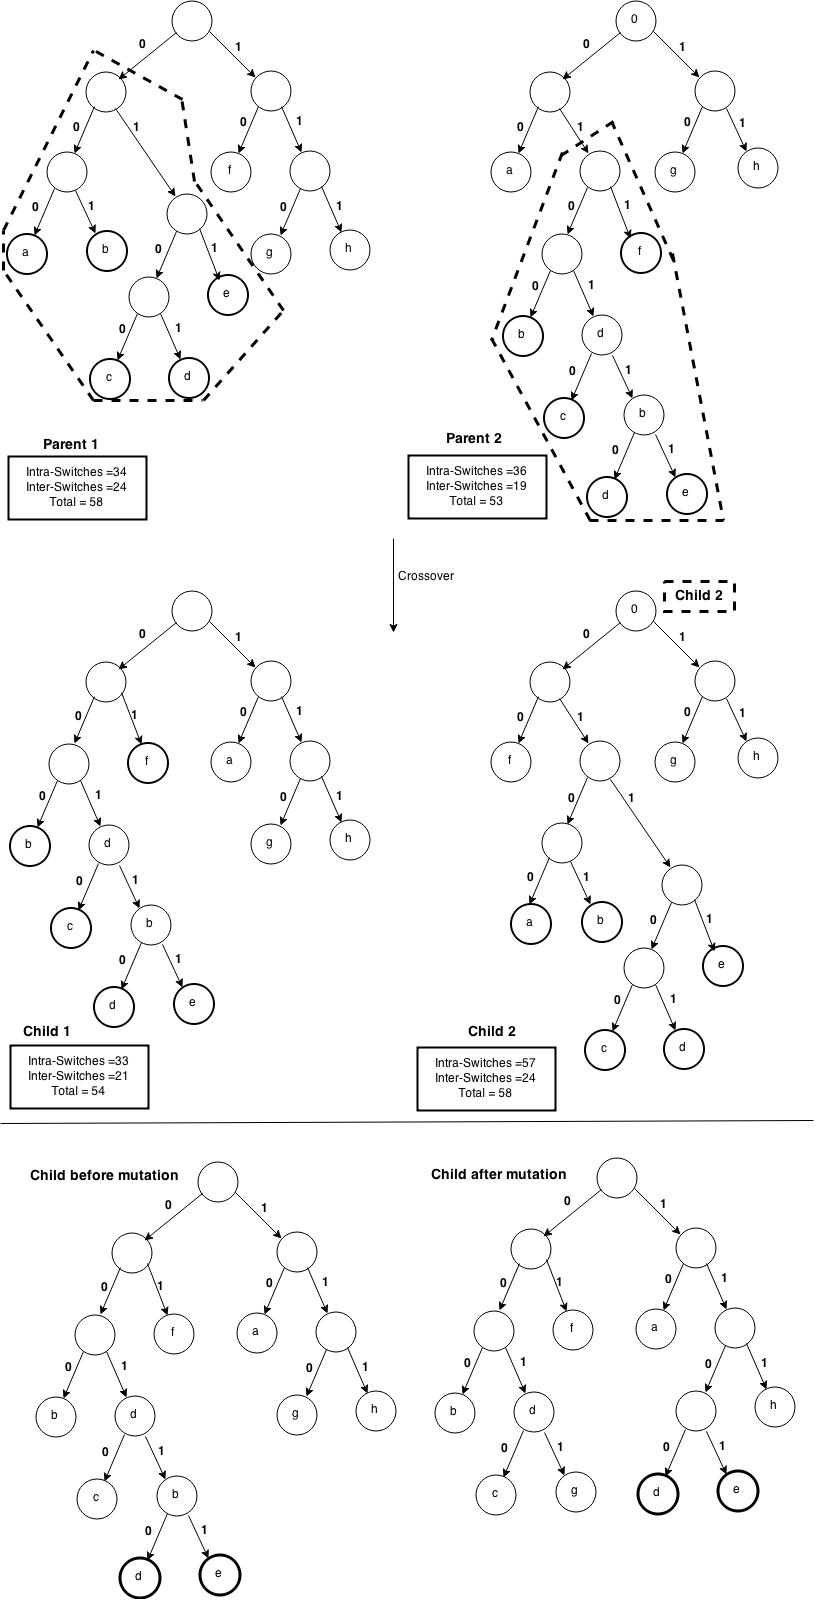
\includegraphics[width=400pt,height=545pt]{Images/Drawing1-1.jpg}
\caption{The Crossover operator}
\end{center}
\label{Fig1}
\end{figure}
\begin{figure}[tbph]
\begin{center}
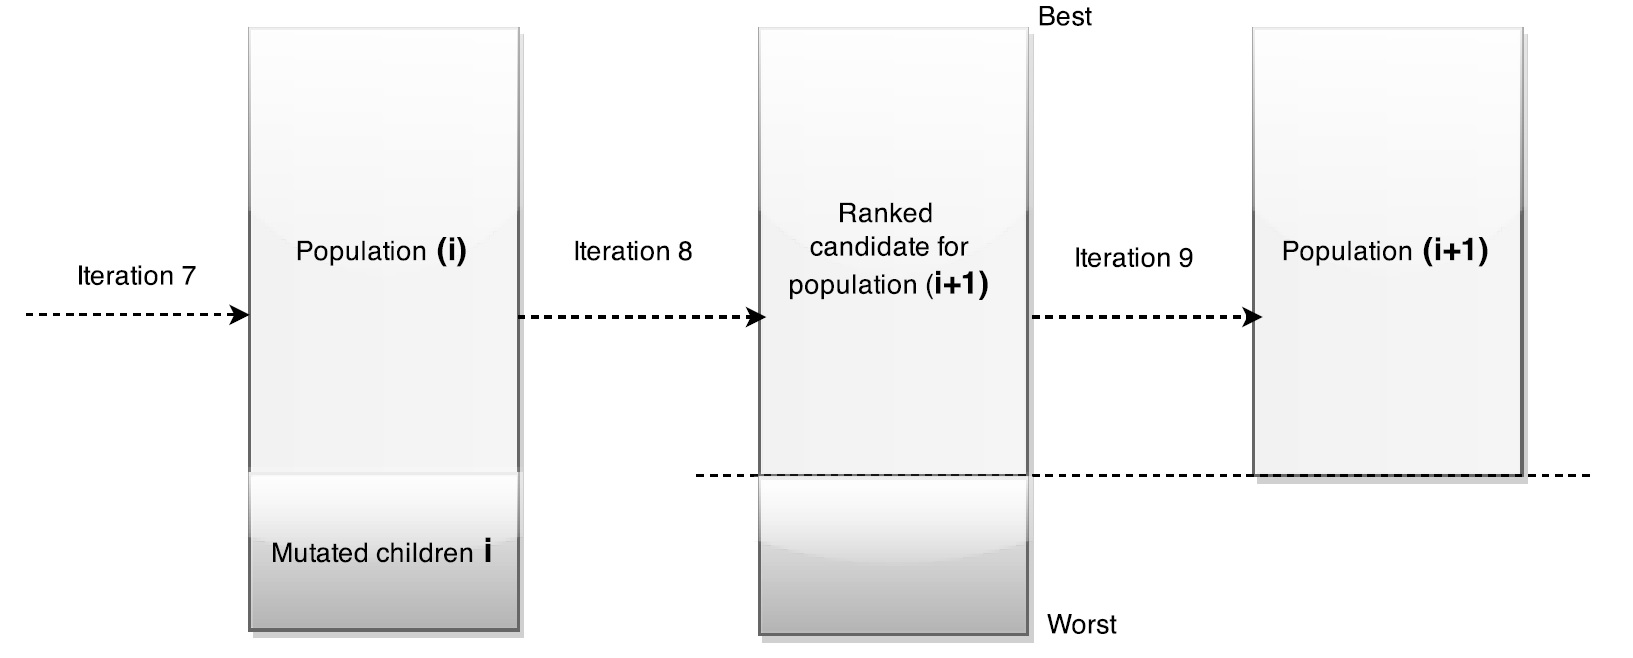
\includegraphics[width=350pt,height=170pt]{Images/Drawing3.jpg}
\caption{Population update for genetic algorithm}
\end{center}
\label{Fig2}
\end{figure}


\section{Experiments and Comparison}



The effectiveness of the approach has been evaluated with different real genomic biological data, these genomes were downloaded from a recent version of The National Center for Biotechnology Information (NCBI) available on $(http://www.ncbi.nlm.nih.gov)$ \cite{pruitt2009ncbi}. We focused on the sequences alone, ignoring any header and any other exogenous information. In table 3, the different data sets are described with the size  of each of them in megabytes (MB) and the references on the biological data bank.

\begin{table}[!thpb]

\small
\label{table3}
\caption{Datasets description}
%\begin{center}
\centering
\begin{tabular}{c  c  c c}
\toprule
$\textbf{Data sets}$ &$\textbf{Name}$ &	$\textbf{Size (MB)}$ &	$\textbf{Reference}$ \\\hline
Genome 1& Mycobacterium smegmatis &  6.66 & CP009496  \\\hline

Genome 2& Amycolatopsis benzoatilytica & 8.30 & NZ\_KB912942 \\\hline

\multirow{2}{*}{Genome 3}&Mycobacterium rhodesiae& \multirow{2}{*}{6.11} & \multirow{2} {*}{CP003169}\\ 
&NBB3& &\\
\hline

\multirow{2}{*}{Genome 4 }&Streptomyces bottropensis& \multirow{2}{*}{8.54} &
\multirow{2}{*}{NZ\_KB911581} \\ 
& ATCC 25435 \\
\hline
    
\multirow{2}{*}{Genome 5}&Mycobacterium smegmatis& \multirow{2}{*}{ 6.66} &\multirow{2}{*}{CP009494             } \\ 
&str. MC2 155 \\
\hline

\multirow{2}{*}{Genome 6}&Mycobacterium smegmatis& \multirow{2}{*}{6.76} &\multirow{2}{*}{NZ\_KI421511}\\   &MKD8& &\\
\hline
    
Genome 7& Bradyrhizobium WSM471&  7.42 &NZ\_CM001442\\\hline

\multirow{2}{*}{Genome 8}&Amycolatopsis thermoflava&  \multirow{2}{*}{8.27} &\multirow{2}{*}{NZ\_CM001442}\\   &N1165 & \\
\hline

\multirow{2}{*}{Genome 9}&Bacillus thuringiensis&   \multirow{2}{*}{5.74} &\multirow{2}{*}{ NZ\_CM000747 }\\    &Bt407&\\
\hline    

\multirow{2}{*}{Genome 10}&Bacillus thuringiensis& \multirow{2}{*}{6.03} &\multirow{2}{*}{ NZ\_CM000748}\\    &serovar thuringiensis& \\
\hline
    
\multirow{2}{*}{Genome 11}&Pseudomonas aeruginosa& \multirow{2}{*}{6.48} &\multirow{2}{*}{NZ\_AFXI01000001}\\    &9BR&\\
\hline
    
\multirow{2}{*}{Genome 12}&Bacillus thuringiensis&  \multirow{2}{*}{5.97} &\multirow{2}{*}{ NZ\_CM000753}\\    &serovar berliner ATCC &\\
\hline
    
\multirow{2}{*}{Genome 13}&Bacillus thuringiensis& \multirow{2}{*}{5.75} &\multirow{2}{*}{ NZ\_CM000750 }\\    &serovar pakistani&\\
\hline
    
\multirow{2}{*}{Genome 14}&Pseudomonas aeruginosa& \multirow{2}{*}{6.28} &\multirow{2}{*}{CP006982}\\    &LES400&\\
\hline

\multirow{2}{*}{Genome 15}& Mus musculus & \multirow{2}{*}{25.58} &\multirow{2}{*}{GL456087}\\  &chromosome 1&\\
\hline

\multirow{2}{*}{Genome 16}& Danio rerio & \multirow{2}{*}{56.14} &\multirow{2}{*}{CM002885}\\ & chromosome 1 &\\
\hline
\multirow{2}{*}{Genome 17}&Homo sapiens & \multirow{2}{*}{76.64 } &\multirow{2}{*}{  CM000680  }\\    & chromosome 18 &\\
\hline
\multirow{2}{*}{Genome 18}&Homo sapiens & \multirow{2}{*}{99.94} &\multirow{2}{*}{CM000684   }\\ & chromosome 22&\\
\hline
%\bottomrule
\end{tabular}
%\end{center}
\end{table} 

\begin{table}[h]
\renewcommand{\arraystretch}{1.1}
\small
\label{table4}
\caption{Comparison of performance among classical Huffman code, CCA, and OCCA without penalty}
%\begin{center}

\begin{tabular}{c  c c  c c  c c}
\hline
 & Huffman Algorithm & P \\\hline
\\\hline
Genome 1& 18.16 & 10.05 & 44.65 \\\hline
Genome 2& 24.66 &  15.63 & 36.61 \\\hline
Genome 3&18.46 &  10.66&  42.25\\\hline
Genome 4&25.18&16.26& 35.42\\\hline
Genome 5& 19.24& 16.08 &16.42 \\\hline
Genome 6& 19.61&14.96&23.71\\\hline
Genome 7& 22.40 &13.21&41.02\\\hline
Genome 8&23.87 & 17.70 &25.84\\\hline
Genome 9&17.66 &10.04&43.14\\\hline
Genome 10& 18.14 &9.89& 45.47 \\\hline
Genome 11&19.63&11.48&41.51 \\\hline
Genome 12& 17.59&11.86&32.57 \\\hline
Genome 13& 17.39&10.93&37.14\\\hline
Genome 14&18.53 &11.64&37.18 \\\hline
Genome 15&78.19 &50.60&35.28 \\\hline
Genome 16& & & \\\hline
Genome 17& & & \\\hline
Genome 18& & & \\\hline
%\bottomrule
\end{tabular}
%\end{center}
\end{table}
\section{Conclusion}
In this paper we described how the genetic algorithm can be used to improve the power consumption in biological data transmission. The advantage of the proposed approach is that it minimise considerably the number of switches with affect directly the power consumption for data transmission. In this paper, we identified genetic
algorithm as a potential method to optimise the total number of inter- and intra-switches. The Genetic algorithm start by generating a set of feasible solutions (trees), each one contain a set of codewords. After that, the approach uses the natural genetic operators to improve the quality if the solutions by generating new solution. the evolution of the population is controlled by the number of switches both inter- and intra-switches. 
The proposed approach is applied to biological data sets with different sizes from small genome to a human chromosome. The approach has been compared with the classic Huffman code. The results show that
the proposed approach improves the power consumption rate considerably. The experiment shows that the proposed approach improves Huffman code in the best case with $best$,  $average$ in the average case, and $worst$ case. For the future we hope to improve the allocation of codewords to different frequencies in orderer to improve the total number of switches.

%% The Appendices part is started with the command \appendix;
%% appendix sections are then done as normal sections
%% \appendix

%% \section{}
%% \label{}

%% If you have bibdatabase file and want bibtex to generate the
%% bibitems, please use
%%
%%  \bibliographystyle{elsarticle-num} 
%%  \bibliography{<your bibdatabase>}

%% else use the following coding to input the bibitems directly in the
%% TeX file.

\section*{References}
\bibliographystyle{elsarticle-num}
\bibliography{mybib}
\end{document}
\endinput
%%
%% End of file `elsarticle-template-num.tex'.
